\documentclass{beamer}
\usetheme{CollegeStation}

\usepackage{subfigure}
\usepackage{bussproofs}
\usepackage{listings}

\newcommand{\comment}[1]{}

\begin{document}
\title{Steve: A Network Protocol Specification Language}
\author{Jasson Casey, Michael Lopez}
\date{\today} 

\frame{\titlepage} 

\frame{\frametitle{Table of contents}\tableofcontents} 

\section{Background}
\subsection{Motivation}

\frame{\frametitle{Robust Networks are Important}
\begin{itemize}
   \item Hard to find absence of networking
   \item World industries are dependent
\begin{figure}[t]
   \centering
   \subfigure {
   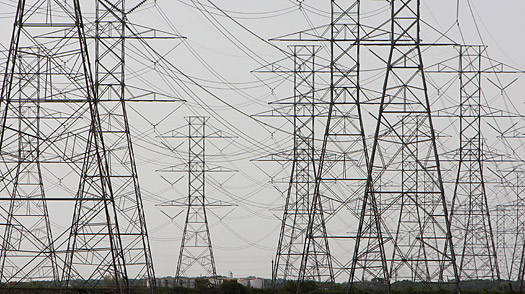
\includegraphics[width=.40\textwidth]{figs/grid.jpg}
   }
   \subfigure {
   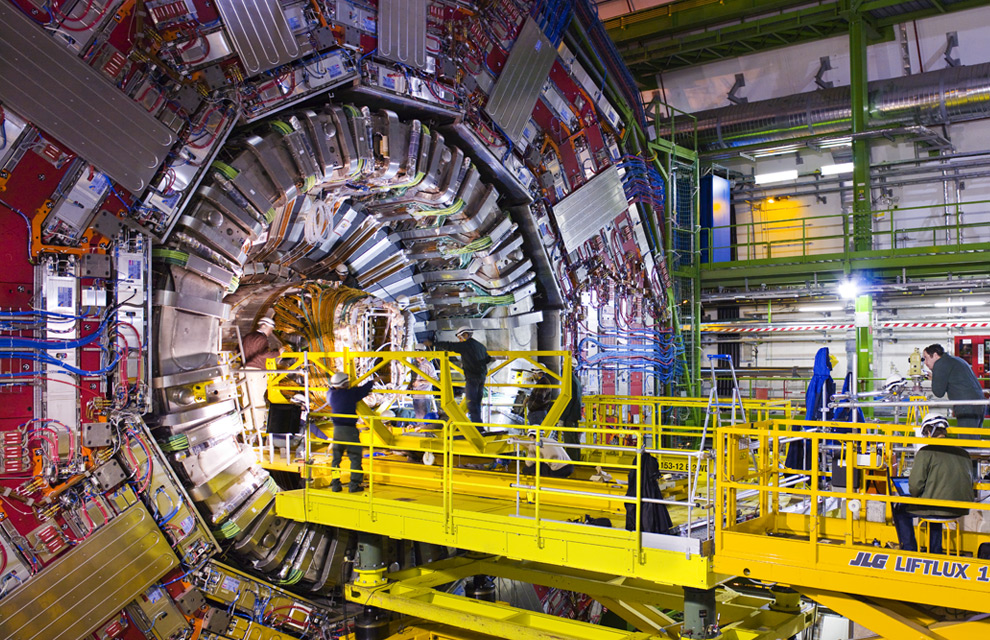
\includegraphics[width=.40\textwidth]{figs/lhc.jpg}
   }
\end{figure}
   \item Getting is right is worth something ...
   \begin{itemize}
      \item \$2.1 Trillion USD in 2012
      \item Insight Research Corp.
   \end{itemize}
\end{itemize}
}

\frame{\frametitle{Implementing Protocols is Hard}
\begin{itemize}
   \item Mature protocols
   \item Experienced engineers
   \item Recent mistakes
\end{itemize}
\begin{center}
   \begin{tabular}{|c|c|c|c|c|}
   \hline
   Age & Protocol & Vendor & Bug Date & US CERT \# \\ \hline
   \hline
   1985 & Bootp & Apple & 2006 & 77628 \\ \hline
   1990 & 802.1q VLAN & Cisco & 2006 & 821420 \\ \hline
   1981 & ICMP & Cisco & 2007 & 341288 \\ \hline
   1985 & NTPD & GNU & 2009 & 853097 \\ \hline
   1998 & OSPFv2 & Quagga & 2012 & 551715 \\ \hline
   \end{tabular}
\end{center}
}

\frame{\frametitle{Complexity is Increasing}
\begin{figure}[t]
   \begin{center}
   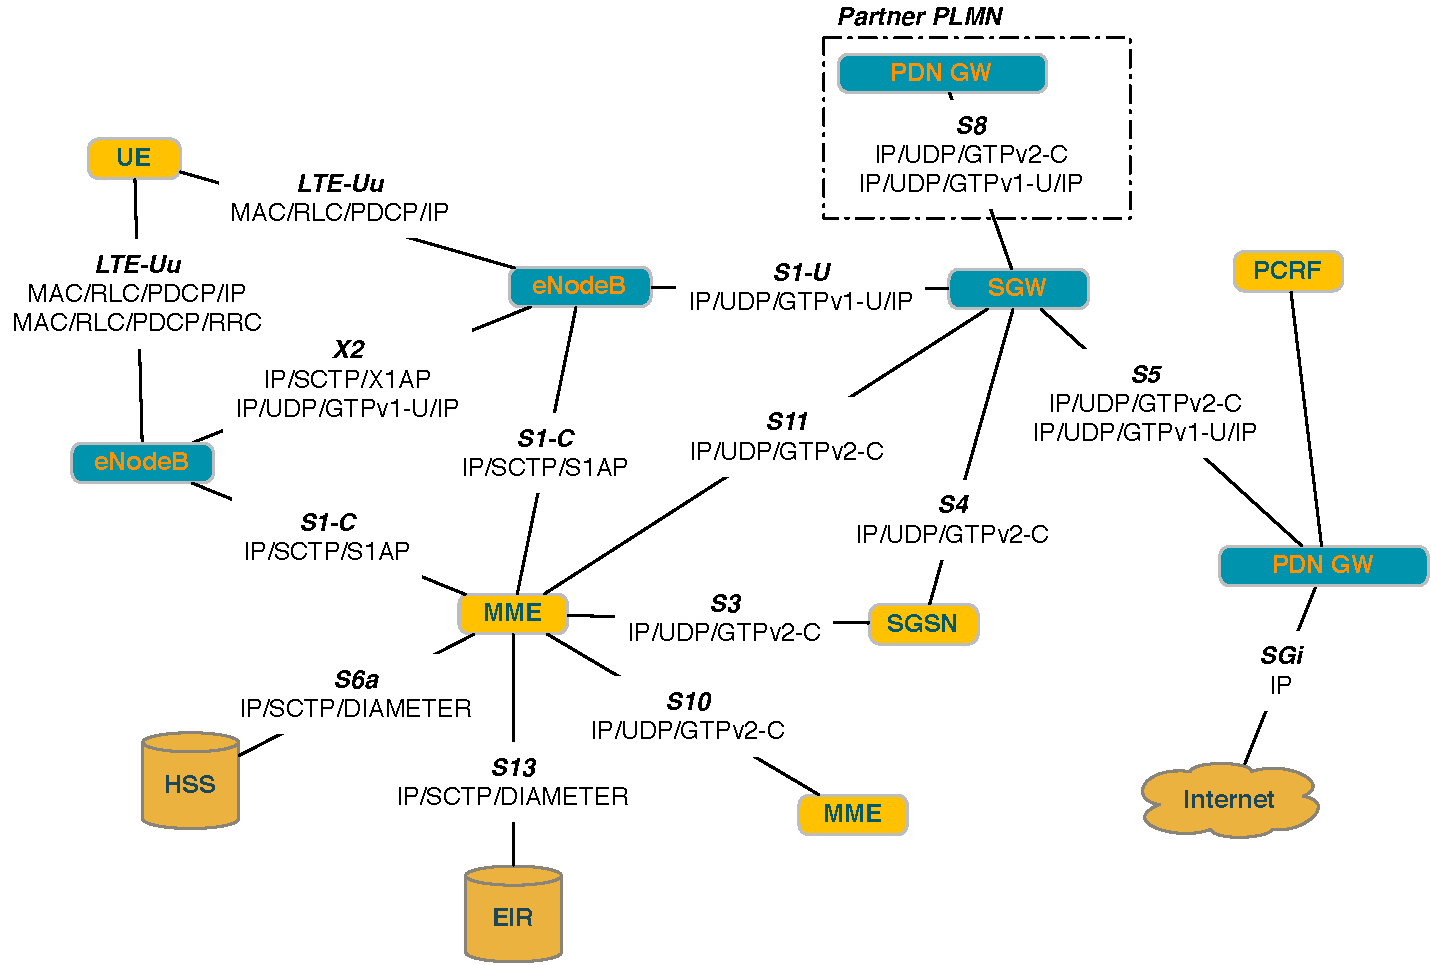
\includegraphics[width=.90\textwidth]{figs/LTE_Arch.pdf}
   \end{center}
\end{figure}
}

\subsection{Existing Work}

\frame{\frametitle{Prior Work}
\begin{itemize}
   \item PacketTypes
      \begin{itemize}
      \item McCann et al., SIGGCOMM 2000
      \end{itemize}
   \item DataScript
      \begin{itemize}
      \item Back, Generative Programming and Component Engineering 2002
      \end{itemize}
   \item Binpac
      \begin{itemize}
      \item Pang et al., SIGCOMM Internet Measurement 2006
      \end{itemize}
   \item PADS/ML/C
      \begin{itemize}
      \item Mandelbaum et al., POPL 2007
      \end{itemize}
\end{itemize}
}

\section{Contribution}

\subsection{Network Protocol Architecture}



\subsection{Steve: A Network Protocol Specification Language}

\frame{\frametitle{Language Terms}
$t::=$   $t$ $t$
   $|$ $\lambda$x$.t$
   $|$ if $t$ then $t$ else $t$
   $|$ $t$ as T
   $|$ let x = $t$ in $t$
   $|$ $\{ x_{i}=t_{i}^{i\in1..n}\}$
   $|$ $t$.x
   $|$ nil
   $|$ cons t t
   $|$ array $t$ $t$
   $|$ uint $t$ $t$
   $|$ pad $t$
   $|$ pdu $t$
   $|$ enum $t$\\

   $\tau::=$ Nat $|$ Char $|$ Bool $|$ Unit $|$ $\tau \rightarrow \tau$ 
            $|$ $[\tau]$ $|$ $\tau ? t$

   $\sigma::=$ $\tau$ $|$ $\alpha$ $|$ $\forall \alpha . \sigma$
}

\frame{\frametitle{Type Constructors}

array $t_1$ $t_2$\\
$t_1=$ expression defining the type contained in the array\\
$t_2=$ expression defining the initial/default value of the array\\
 
uint $t_1$ $t_2$\\
$t_1=$ expression defining the number size of this uint in bits\\
$t_2=$ expression defining the initial/default value of this type\\

pad $t$\\
$t=$ expression defining the number of bits to skip\\

}

\subsection{A Theory of Steve}

\frame{\frametitle{Predicate Introduction}
\begin{itemize}
   \item $\Delta$ - set of known facts
   \item conditional terms introduce predicates
   \item evaluate sub-terms using new fact established by predicate
\end{itemize}
 
\begin{prooftree}
   \scriptsize
   \def \fCenter{\ \vdash\ }
   \RightLabel{\textbf{T$_{if}$}}
   \AxiomC{$\Delta | \Gamma \fCenter\ t_1 : Bool$}
   \AxiomC{$\Delta,\{t_1\} | \Gamma \fCenter\ t_2 : \tau$}276 \AxiomC{$\Delta,\{\neg t_1\} | \Gamma \fCenter\ t_3 : \tau$}
   \TrinaryInfC{$\Delta | \Gamma \fCenter\ $ if $t_1$ then $t_2$ else $t_3 : \tau$}
\end{prooftree}
}

\frame{\frametitle{Dependency Elimination}
\begin{itemize}
   \item deduce dependency from known facts
   \item eliminate dependency in resulting type
\end{itemize}
 
\begin{prooftree}
   \scriptsize
   \def \fCenter{\ \vdash\ }
   \RightLabel{\textbf{T$_{DepElim_1}$}}
   \AxiomC{$\Delta | \Gamma \fCenter\ t : \tau ? \delta$}
   \AxiomC{$\Delta \vDash \delta$}
   \BinaryInfC{$\Delta | \Gamma \fCenter\ t : \tau$}
\end{prooftree}
}

\frame{\frametitle{Dependency Deferral}
\begin{itemize}
   \item use of type without proof of dependency
   \item rewrite term using conditional
   \item eliminate dependency of type
\end{itemize}
 
\begin{prooftree}
   \scriptsize
   \def \fCenter{\ \vdash\ }
   \RightLabel{\textbf{T$_{DepElim_2}$}}
   \AxiomC{$\Delta | \Gamma \fCenter\ t : \tau ? \delta$}313 \AxiomC{$\Delta \nvDash \delta$}
   \BinaryInfC{$\Delta | \Gamma \fCenter\ t : \tau ? \delta \rightsquigarrow$ if $
   \delta$ then $t$ else $error : \tau$}
\end{prooftree}
}

\subsection{Steve's interpreter}

\section{Results}

\comment{
\frame{\frametitle{Simple Example}
\begin{verbatim}
 rcv :: ARP -> Unit
 rcv pkt as ARP =
    if pkt.type == Request
       then send pkt.mac ( arp_who_has pkt.ip )
       else arp_update pkt.mac pkt.ip
 
 rcv :: IPv4 -> Unit
 rcv pkt as IPv4 =
    if pkt.ttl == 0
       then send pkt.src ( make_dst_unreach pkt )
       else fwd ( dec_ttl pkt )
    
 rcv :: EtherII -> Unit
 rcv pkt as EtherII = 
    rcv pkt.payload  
\end{verbatim}
}
}

\section{Conclusions}
\frame{\frametitle{Conclusion}
\begin{itemize}
\item
\end{itemize}
}
\end{document}

